The getwork RPC method was developed and written into Bitcoin Core as all the other RPCs, in this way anyone who was running a full node was able to use it to mine new blocks.\\
By the way, even if Bitcoin was just born (3rd January 2009), the first mining pools started to appear (\textit{slushpool} was born in 2010 as well). Due to the nature of the RPC method, it had been used also into a pooled mining context: it could be sent over HTTP transport layer, providing an elegant way for the pool operators to get and distribute new jobs to miners who were joining the pool.\\
In the context of pooled mining, where every single miner had to communicate with the pool server, the exploitation of some protocol extensions seemed to be particularly useful in that scenario.\cite{bitcoinGetworkBitcoin}\\
More specifically, when getting new work, miners could send a \textbf{X-Mining-Extensio\\ns} header with a space-delimited list of supported extensions:
\begin{itemize}
\item 
\textbf{Hostlist} 

The server may include a X-Host-List header with a list of available servers formatted in JSON as an array of objects with server details. The field "host" specifies the server's hostname or IP address, "port" specifies a TCP port, and "ttr" is "time to return". If you use server with non-zero ttr you should try to return to the server with 0 ttr after this number of minutes. 

\underline{Example:} 
\begin{verbatim}
X-Host-List: [{"host":"server.tld","port":8332,"ttr":0},
{"host":"backup.tld","port":8332,"ttr":20}]
\end{verbatim}


This string says that "server.tld" is the main server. When you detect connection problems, you need to try the next server - "backup.tld" for 20 minutes and then try to switch back to "server.tld". If the main server is still offline you should continue to use "backup.tld" for another 20 minutes.

\item 
\textbf{Longpoll}\label{sec:longpolling}

If mining pool does supports Long Polling, it should include a X-Long-Polling header with a relative or absolute URI. The absolute URI may specify a different port than the original connection. Miner must start a request to long polling URI with GET method and same basic authorization as on main connection. This request is not answered by server until it wishes to expire current block data, and new data is ready. The answer is the same as getwork on the main connection. Upon receiving this answer, miner should drop current calculation in progress, discard its result, and start working on received data and make a new request to a long polling URI. There is a 60 second limit before new work should be requested (the normal way) regardless of response from longpoll (though this may be overridden by the rollntime extension below).

\item 
\textbf{Noncerange} 

In addition to X-Mining-Extensions, the miner should also send X-Mining-Hashrate, with an integer value of expected hashrate measured in full hashes per second. The server may then add an additional field to the JSON response, "noncerange", which contains two 32-bit integers specifying the starting and final nonce the miner is allowed to scan. While both values are given in big endian, miners should iterate over the range in their native 32-bit integer type (SHA256 works with 32-bit integers, not character data). The miner should implement rollntime by starting from the first nonce in the range every second.

\underline{Example:} 
\begin{verbatim}
"noncerange": "000000001fffffff"
\end{verbatim}
\underline{Response:} 
\begin{verbatim}
solution: "...dddddd1f..."
\end{verbatim}
A very interesting discussion about the noncerange extension can be found on Bitcoin Talk Forum \cite{bitcointalkMiningProtocol}.

\item 
\textbf{RollNtime}
If the getwork response includes a "X-Roll-Ntime" header with any value other than "N" or the null string, the miner may (within reason) change the ntime field in addition to the nonce. The server may send a value of "expire=<N>", where <N> is an integer number of seconds it is willing to accept the other headers for. Note that if the "X-Roll-NTime" header is NOT present in a work response, that work may NOT be rolled, even if earlier work from the same server allowed it. Also note that the headers of a share submission should not influence the behavior of work. More specifically, if a share submit does not have the header, it should not disable rollntime for the current work (which did).\\\\
To investigate more deeply, an official discussion about the RollNtime extension can be found on Bitcoin Talk Forum \cite{bitcointalkXRollNtimeExtension}.
\end{itemize}

\begin{figure}[h!]
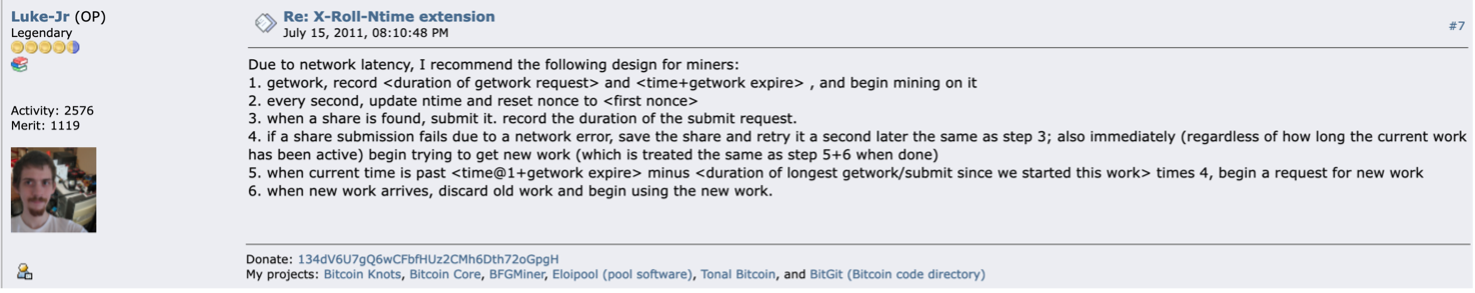
\includegraphics[width=1\textwidth, right]{Figures/getwork/getwork6.png}
\caption{Luke-Jr mining operations recommendations, on \textit{Bitcoin Talk Forum}}
\label{fig:getwork6}
\end{figure}

